Als   Ausgangspunkt  der   Reglerdimensionierung   dient  die   Schrittantwort
der  Strecke,   aus  welcher   die  Verts\"arkung   $K_s$  der   Strecke,  die
Verz\"ogerungszeit  $T_u$ und  die Anstiegszeit  $T_g$ abgelesen  werden.  Bei
unserem Tool werden diese Werte als Eingabeparameter verwendet.

Wir werden in diesem Bericht folgende Strecke als Beispiel nehmen:
\begin{figure}[h! width=\pagewidth]
    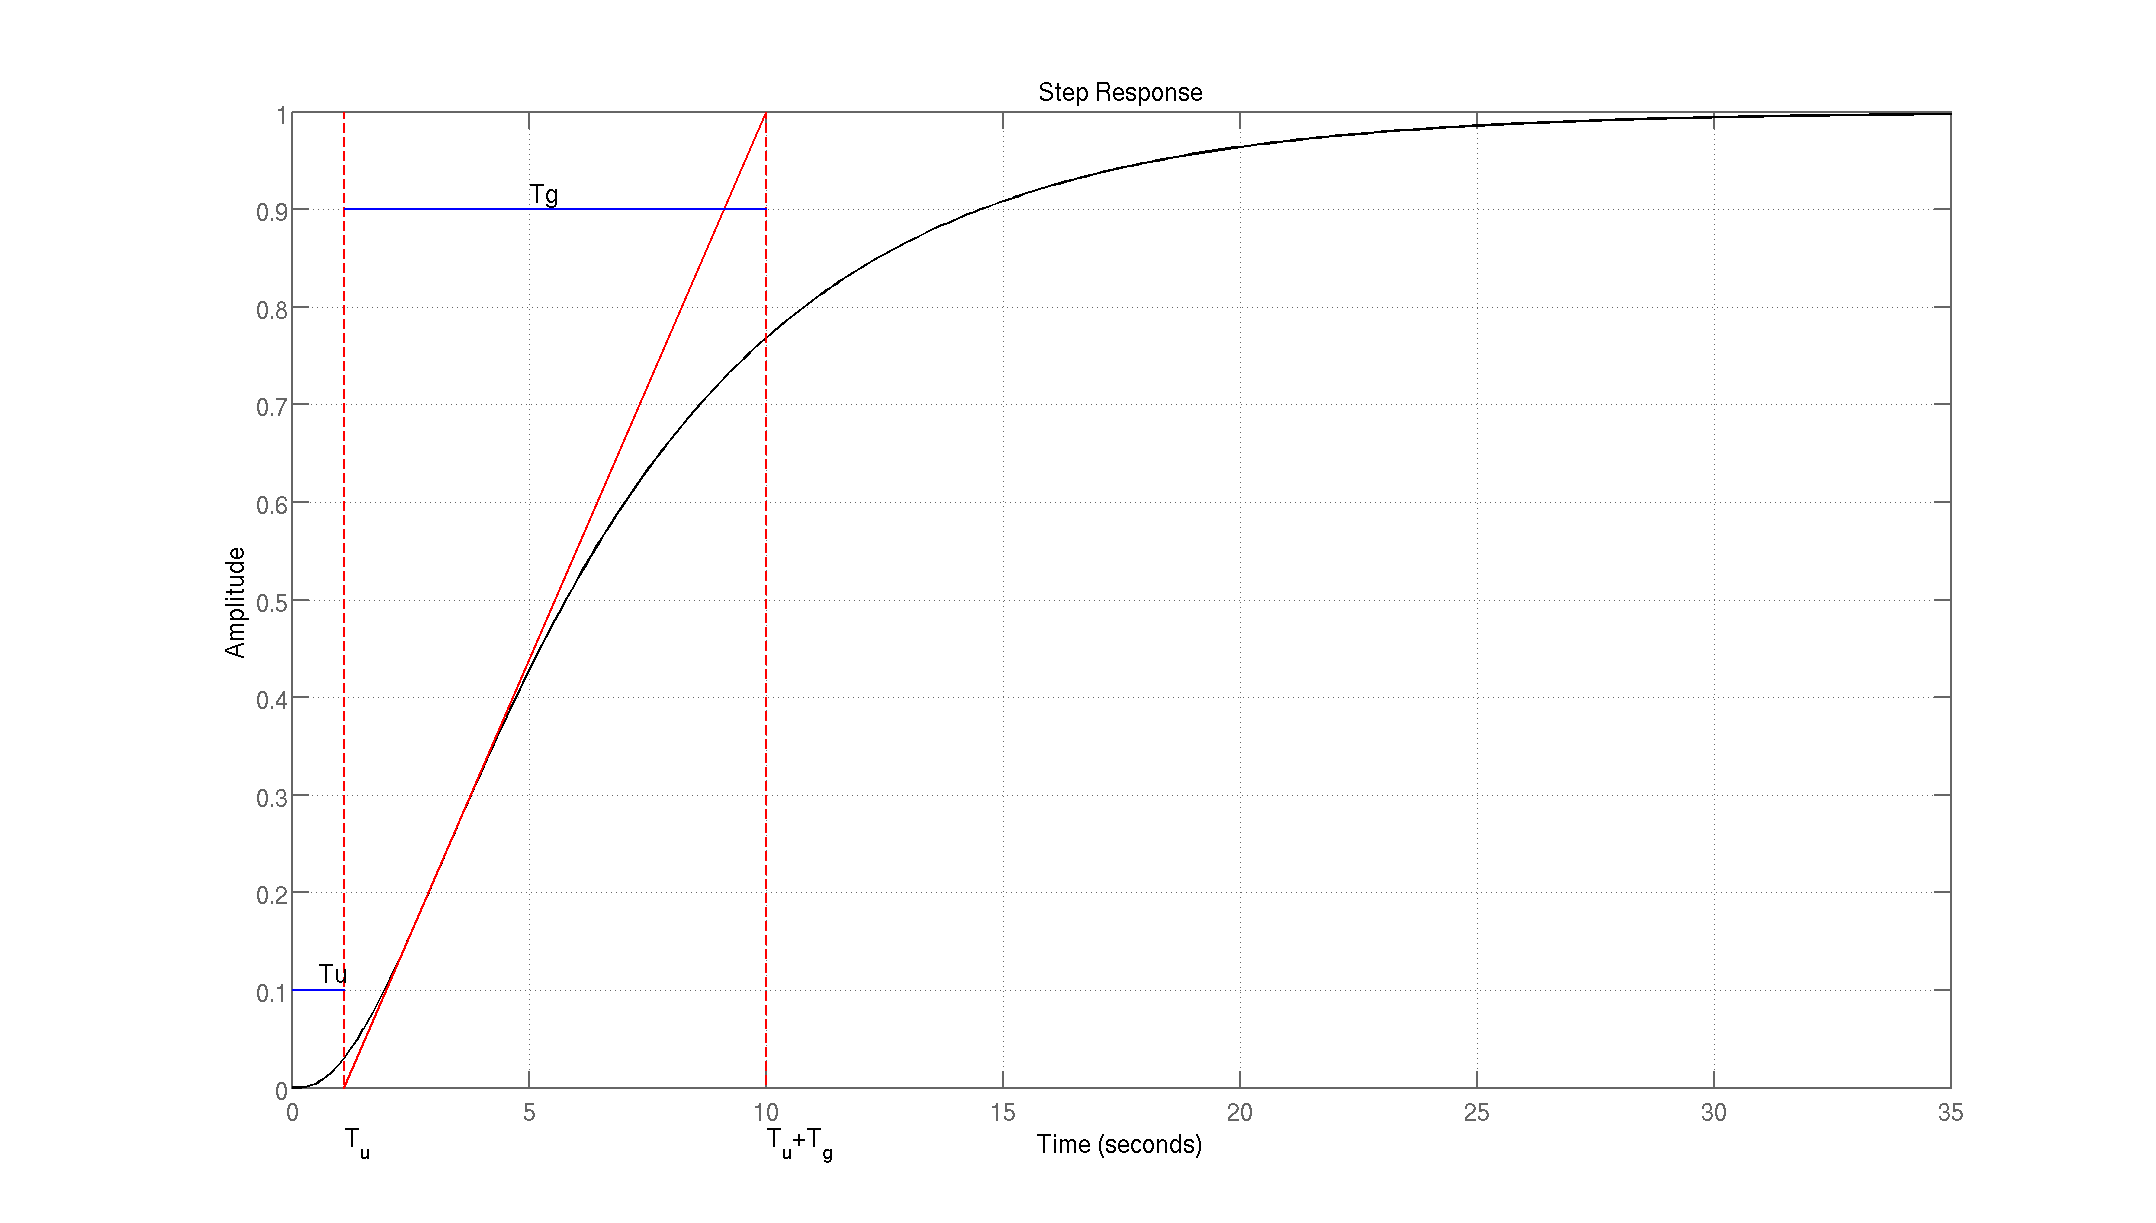
\includegraphics[width=\textwidth]{images/streckeSchrittantwort.png}
    \caption{%
    Schrittantwort der  Beispielstrecke (schwarz), Wendetangende  (rot), $T_u$
    und $T_g$ (blau)%
    }
    \label{fig:plant_step}
\end{figure}

Der  geschlossene   Regelkreis  soll  schlussendlich  maximal   etwa  $16.3\%$
\"uberschwingen.

Ausmessen der Schrittantwort ergibt:
\begin{itemize}
    \item
        $K_s = \SI{2}{\second}$
    \item
        $T_u = \SI{1.1}{\second}$
    \item
        $T_g = \SI{8.9}{\second}$
\end{itemize}

Da die Reglerdimensionierung vom \emph{Frequenzgang} einer Strecke ausgeht und
nicht von deren  Schrittantwort, besteht der n\"achste Schritt  nun darin, aus
den obigen Werten den Frequenzgang der Strecke zu bestimmen. Dies erledigt die
Methode  \code{p\_sani}\footnotemark[1],   welche  uns  die  Werte  f\"ur  die
\"Ubertragungsfunktion  der  Strecke  liefert.  \todo{Allenfalls  Verweis  auf
Softwareteil  f\"ur Erkl\"arungen  zu sani-Methode.}   In unserem  Fall ergibt
dies folgendes Polynom:

\footnotetext[1]{%
    Die  Methode  \code{p\_sani}  wurde  zu  Beginn  des  Projektes  in  einer
    Matlab-Implementation  zur Verf\"ugung  gestellt  und anschliessend  f\"ur
    unser Tool in Java \"ubersetzt.
}

\begin{gather} \label{eq:transfer:plant}
    \begin{split}
        H_s (s) & = K_s
                  \cdot \frac{1}{1 + s \cdot T_1}
                  \cdot \frac{1}{1 + s \cdot T_2}
                  \cdot \frac{1}{1 + s \cdot T_2}                     \\
                & = 2
                  \cdot \frac{1}{1 + s \cdot \SI{0.4134}{\second}}
                  \cdot \frac{1}{1 + s \cdot \SI{1.4894}{\second}}
                  \cdot \frac{1}{1 + s \cdot \SI{5.3655}{\second}}
    \end{split}
\end{gather}

Mit einem  geeigneten Tool  kann man sich  den dazugeh\"origen  Plot erstellen
lassen.

\begin{figure}[h! width=\pagewidth]
    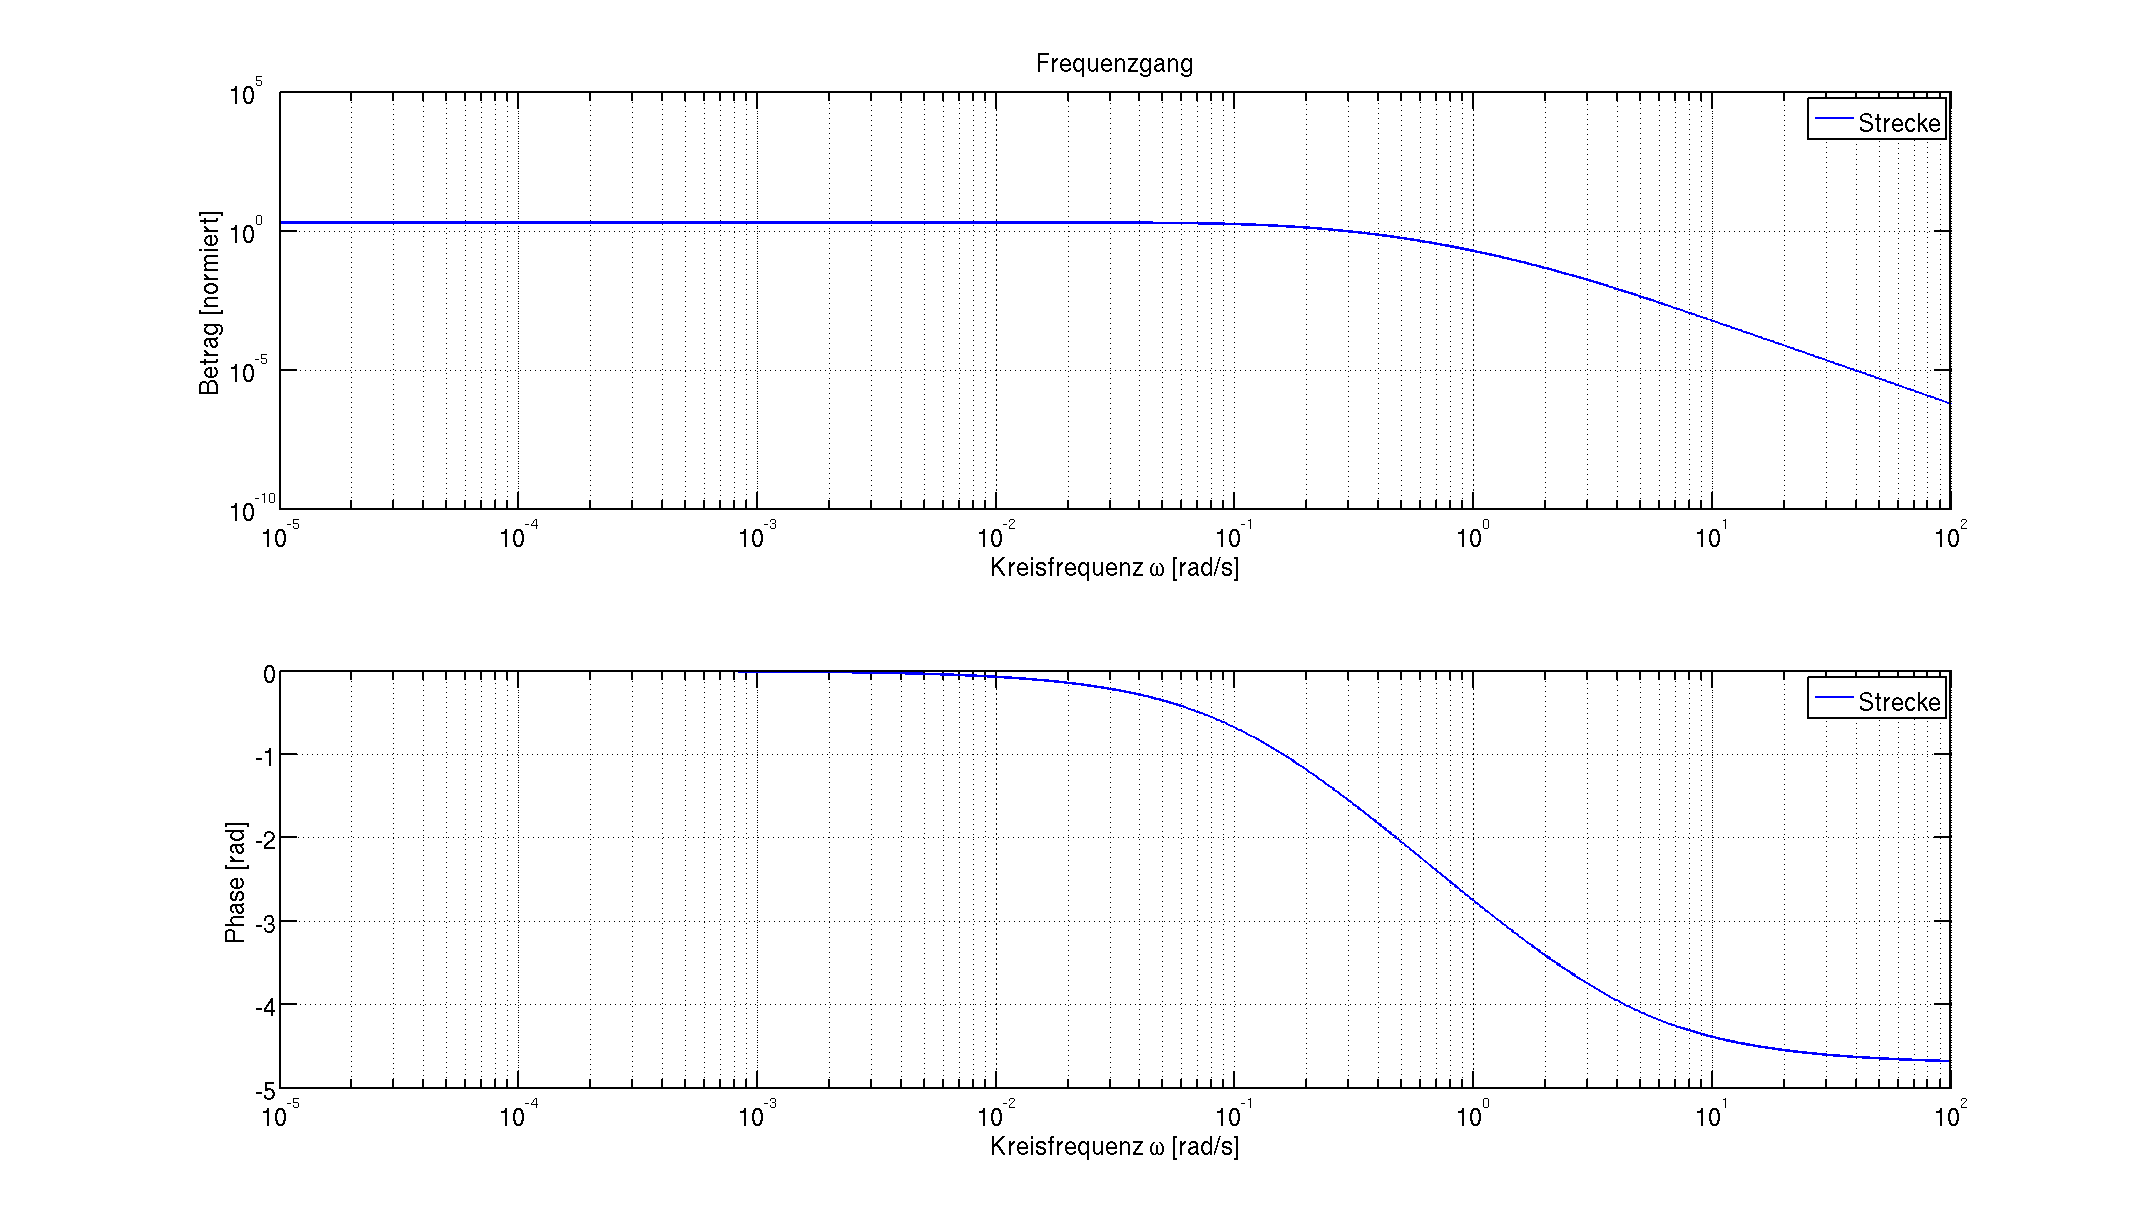
\includegraphics[width=\textwidth]{images/streckeFrequenzgang.png}
    \caption{%
        Frequenzgang der Strecke%
    }
    \label{fig:plant_freq}
\end{figure}

Somit  ist  der Frequenzgang  der  Strecke  bekannt  und  man kann  mit  einer
geeigneten Methode den Regler dimensionieren.
